\chapter{Mecanismos de sincronización en redes de computadores}

En este capítulo se detalla las características principales de los mecanismos 
empleados para la sincronización de equipos en red. Además se introducen los 
protocolos estándar más extendidos como \gls{ntp} o \gls{ptp} para llegar a una 
explicación más detallada sobre la extensión de \gls{ptp} conocida como 
\acrlong{wr}.

Los requisitos demandados por las aplicaciones que necesitan de algún mecanismo 
de sincronización son bastante heterogéneos. Esto es fácilmente entendible si 
se piensa en dos ejemplos de aplicaciones concretos: mantener la hora de 
sistema en los computadores de una red de propósito general, y hacerlo en los 
elementos de una fabrica de montaje de alta precisión.
En ambos escenarios se necesita de un mecanismo que permita mantener una misma 
noción de tiempo en los elementos del sistema, sin embargo en el primer 
escenario se puede tolerar un nivel de error que sería inaceptable en el 
segundo.
En otras aplicaciones, lo realmente importante es que todos los nodos de la red 
realicen una misma cuenta del tiempo, es decir, que la duración de un segundo 
sea lo más parecida en todos los nodos, sin importar tanto la fecha y la hora. 
En estos casos la sincronización se realiza mediante la distribución de una 
señal de reloj que se utiliza en los contadores internos de cada nodo. 

\section{Referencias de tiempo y frecuencia}

\section{Fuentes de ruido y desfase}

3.1.1 accuracy: The mean of the time or frequency error between the clock under 
test and a perfect
reference clock, over an ensemble of measurements. Stability is a measure of 
how the mean varies with
respect to variables such as time, temperature, and so on. The precision is a 
measure of the deviation of the
error from the mean.

\section{Network Time Protocol}

\textit{\acrlong{ntp}} \cite{Mills1991} es un protocolo estándar de red 
empleado para la sincronización de relojes en computadores conectados mediante 
redes conmutadas, que fue diseñado por David L. Mills de la Universidad de 
Delaware. Su uso se demostró públicamente por primera vez en 1979, en lo que 
sería una prueba de enlace satelital transatlántico para varios servicios de 
Internet. Posteriormente, en 1985 se implementó NTPv0 para sistemas tipo Unix 
donde la estructura para la cabecera y los cálculos para el tiempo de ida y 
vuelta (o \textit{round-trip time}) y el desfase entre relojes son los que se 
siguen utilizando en la versión actual NTPv4.

Los servidores \gls{ntp} pueden operar en varios modos: \textit{multicast}, 
llamada a procedimiento remoto y simétrico. El modo \textit{multicast} está 
enfocado a redes de área local (\gls{lan}) donde el número de clientes es 
grande y no se necesita de un alto nivel de precisión. En este escenario, uno o 
varios servidores se encuentran continuamente enviando mensajes de difusión 
\gls{ntp} que reciben los clientes que serán los encargados de calcular el 
desfase de su reloj con respecto al del servidor. Los servidores anuncian la 
posibilidad de proveer sincronización pero no aceptan mensajes \gls{ntp} de 
ninguno de los pares.
El segundo modo está pensado para escenarios donde se necesite una gran 
exactitud en la sincronización. Los servidores pueden actuar como cliente 
aceptando la sincronización de otro par (sin proveerla de forma descendente) o 
en modo servidor donde no aceptan ser sincronizados.
Los modos \textit{multicast} y llamada a procedimiento remoto no escalan bien 
en redes grandes de ámbito general como Internet. Para ello, los servidores de 
tiempo deben poder distribuirse de forma dinámica con una topología 
jerarquizada. Para este tipo de modo se emplea la comunicación simétrica donde 
el algoritmo de selección de \gls{ntp} determina el rol de cada uno de los 
servidores en la red.

\subsection{Organización de la red}

La topología de red usada en \gls{ntp} es de tipo jerárquica, donde el índice 
del nivel es un indicativo de la cercanía a la fuente primaria de tiempo. A 
cada nivel de la jerarquía se le denomina estrato. Se comienza a numerar por 0 
y se va sumando 1 por cada nivel de conexión en la jerarquía, es decir, un 
servidor sincronizado a un estrato \textit{n} se encontrará a \textit{n+1} 
saltos de la fuente principal. Este índice indica la distancia a la fuente y no 
necesariamente la calidad del servidor.

\begin{figure}
	\centering
	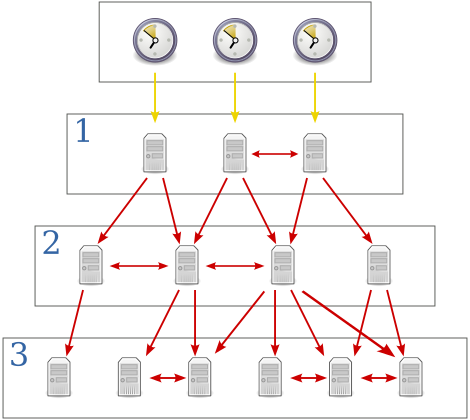
\includegraphics[width=0.7\linewidth]{imagenes/ntp_tree}
	\caption[Esquema de una red de distribución de tiempo usando NTP.]{En este 
	diagrama se 
	muestra una posible red de distribución de tiempo usando NTP. En el estrato 
	0 se hayan las fuentes de reloj de alta estabilidad como GPSDO o relojes 
	atómicos. Estas se conectan directamente a los servidores del estrato 1 que 
	forman los llamados servidores de tiempo primarios. Esta capa provee la 
	hora UTC al resto de los niveles. Como se puede ver se pueden establecer 
	enlaces entre equipos del mismo nivel, además, pueden estar conectados a 
	varios servidores de la capa superior (redundancia). Imagen tomada de 
	\cite{website:imgNTPtree}}
	\label{fig:ntptree}
\end{figure}


El límite superior para un estrato es el 15. Para indicar que un dispositivo no 
está sincronizado se utiliza el valor de estrato 16. El algoritmo \gls{ntp} 
está diseñado para construir una topología con los caminos más cortos hacía los 
servidores del estrato 1 (haciendo uso del algoritmo Bellman-Ford) lo que 
minimiza el tiempo de ida y vuelta acumulado entre los servidores de estrato 1 
y los clientes. A continuación se describen brevemente los estratos más 
relevantes:

\begin{itemize}
	\item \textbf{Estrato 0} \\ A este nivel se encuentran las fuentes de 
	tiempo de alta precisión, entre las que cabe destacar los relojes atómicos 
	o los osciladores disciplinados por GPS (\acrshort{gpsdo}). Generan una 
	señal de un pulso por segundo (\acrshort{pps}) que permite disciplinar el 
	oscilador interno del servidor conectado a la fuente de nivel 0.
	
	\item \textbf{Estrato 1} \\ Lo forman los servidores cuyos relojes se 
	disciplinan directamente con la señal recibida de una fuente de nivel 0 
	logrando una sincronización en torno a unos pocos microsegundos. Además 
	pueden conectarse con otros del mismo nivel para tareas de comprobación de 
	errores o para redundancia.
	
	\item \textbf{Estrato 2 (en adelante)} \\ Los dispositivos de cada estrato 
	se 
	sincronizan con el estrato anterior, pudiendo hacerlo con varios servidores 
	a la vez, y además pueden hacerlo con otros computadores del mismo nivel a 
	fin de mejorar la calidad del servicio.
\end{itemize}

\subsection{Algoritmo}

La figura \ref{fig:ntptree} muestra un esquema de organización típico para una 
red de distribución de tiempo usando \gls{ntp}. Para realizar el cálculo del 
desfase del reloj cliente con respecto al servidor, se emplean una serie de 
paquetes con marcas de tiempo (\textit{timestamps}). El cliente debe iniciar el 
proceso realizando una petición al servidor como muestra la figura 
\ref{fig:ntpts}. El servidor recibe el paquete y lo sella en el instante $T_i$. 
Para realizar los cálculos se emplean siempre las 4 marcas más recientes. Con 
ello se puede realizar el cálculo del tiempo de ida y vuelta ($\delta_i$), y el 
desfase del reloj ($theta_i$) del cliente con respecto al del sevidor en el 
instante de tiempo $T_i$:

\begin{equation}\label{ntprtt}
	\delta_i = (T_{i-2}-T_{i-3}) - (T_{i-1}-T_{i})
\end{equation}\label{ntpoffset}
\begin{equation}
	\theta_i = \frac{(T_{i-2}-T_{i-3}) + (T_{i-1}-T_{i})} {2}
\end{equation}

Hay que tener en cuenta que el servidor no tiene por qué contestar a las 
peticiones del cliente de forma inmediata. El proceso encargado de la gestión 
del servicio \gls{ntp} puede ser interrumpido por otra tarea con más prioridad, 
lo que hace que el tratamiento de las marcas de tiempo no sea determinista.

\begin{figure}
	\centering
	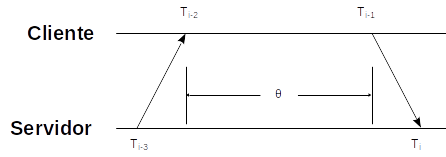
\includegraphics[width=0.7\linewidth]{imagenes/ntp_ts}
	\caption[Cálculo del desfase entre cliente y servidor]{La figura muestra un 
	intercambio de paquetes con marcas de tiempo entre cliente y servidor. Para 
	calcular el tiempo de ida y vuelta se utilizan 4 marcas de tiempo.}
	\label{fig:ntpts}
\end{figure}

\subsection{Rendimiento}

Al ser \gls{ntp} un protocolo que se implementa completamente en 
\textit{software}, no se consigue una gestión determinista para el cálculo del 
desfase entre las dos entidades que se sincronizan. Ello conlleva una 
limitación severa a la exactitud alcanzable mediante el uso de este protocolo 
\incomment{Mejorar esa frase}. Aunque este hecho podría ser tratado mediante el 
uso de sistemas operativos de tiempo real o técnicas que consigan reducir la 
latencia con la que el proceso encargado de la gestión del protocolo \gls{ntp} 
es ejecutado, existe otro factor de diseño que tiene incluso más peso en la 
precisión alcanzable por éste: la asunción de igualdad entre los caminos de ida 
y vuelta para los paquetes enviados por la red de comunicación. En \gls{ntp} se 
considera que el camino de transmisión de los paquetes es simétrico al camino 
de recepción, lo cual es bastante improbable en redes conmutadas con varios 
saltos y múltiples caminos como es el caso de Internet. Todo ello conlleva que 
la exactitud que alcanza este protocolo de forma general, sincronizando dos 
equipos, se sitúe en el orden de los milisegundos llegando a decenas de 
microsegundos en condiciones controladas.
\section{Precision time protocol}

Aunque el desarrollo del protocolo \gls{ntp} supuso un gran avance con respecto 
a las técnicas de sincronización en redes utilizadas anteriormente, la 
exactitud que podía alcanzar dicho protocolo no era suficiente para las 
aplicaciones con requisitos de altas prestaciones como los sistemas de control 
o sistemas de medición distribuidos. Para mejorar el rendimiento se propuso el 
desarrollo de un protocolo denominado \acrlong{ptp}, bajo el estándar 
\acrshort{ieee} 1588-2002 (año de su publicación) \cite{IEEE1588-2008}. 
Actualmente se utiliza la segunda revisión del estándar: IEEE 1588-2008 o 
\gls{ptp}v2, que no presenta compatibilidad con la versión anterior.

\subsection{Arquitectura de red}

El protocolo \gls{ptp} define una arquitectura jerárquica de tipo 
maestro-esclavo. Al igual que en la red \gls{ntp}, el nodo raíz puede estar 
conectado a una fuente estable de tiempo, como un \gls{gpsdo} o un reloj 
atómico, y provee de sincronización al resto de la red. En el caso de \gls{ptp} 
este nodo recibe el nombre de \acrlong{gm}. Los nodos intermedios pueden actuar 
como maestros del nivel siguiente o como nodos finales. A continuación se 
detallan las características más relevantes de los tipos de dispositivos más 
usuales:

\begin{itemize}	
	\item \textbf{\gls{oc}} \\
	Este tipo de nodos se comunican con el resto de la red via una única 
	intefaz de red física de tipo bidireccional que se encarga del intercambio 
	de los paquetes con las marcas de tiempo con el resto de la red. La 
	configuración de \gls{oc} sólo permite una única ejecución del 
	protocolo 
	\gls{ptp} y un único estado de funcionamiento. Así, este tipo de 
	configuración, permite al dispositivo actuar como maestro de la red 
	(\acrshort{gm}) o como reloj esclavo.
	
	\item \textbf{\gls{bc}} \\
	Los dispositivos que actúan como \acrshort{bc} suelen disponer de múltiples 
	puertos físicos que pueden actuar como si fuesen \gls{oc}s pero que 
	comparten una misma referencia de tiempo (recuperada del nodo maestro en el 
	nivel superior). Es decir, uno de los puertos se configurará como esclavo y 
	el resto podrán actuar como puertos maestros para los siguientes nodos de 
	la red.
	
	\item \textbf{\gls{tc}} \\
	La gran diferencia con respecto a los tipos anteriores reside en que los 
	\gls{tc} no se sincronizan con un nodo maestro. Estos actúan como simples 
	repetidores del tráfico entrante, pero modifican el campo de corrección de 
	los mensajes \textit{Follow\_UP o Pdelay\_Resp\_Follow\_UP} para incluir el 
	tiempo de residencia de los paquetes \gls{ptp} en el \gls{tc}. El campo de 
	corrección es usado posteriormente por los \gls{oc} para realizar el ajuste 
	de su reloj interno. 
	Dependiendo del mecanismo empleado para el cálculo del tiempo de 
	propagación se distinguen dos tipos de \gls{tc}: \textit{End-to-end} y 
	\textit{Peer-to-peer}.
\end{itemize}

\subsection{Algoritmo}

En el protocolo \gls{ptp} se distinguen dos fases de ejecución:
\begin{enumerate}
	\item Establecimiento de la jerarquía en la red.
	\item Sincronización de los relojes.
\end{enumerate}

En el arranque del algoritmo \gls{ptp} se espera por un lapso de tiempo a 
recibir mensajes de tipo \textit{Announce} provenientes de algún maestro en la 
red. Si no se reciben mensajes de ese tipo, el nodo asume que es maestro hasta 
que un maestro con mejores prestaciones aparezca en la red. La configuración de 
roles en la red se realiza mediante un algoritmo llamado \gls{bmc}, que utiliza 
varios parámetros como calidad de la fuente de reloj de un nodo o el nivel en 
el que se encuentra de la jerarquía (entre otras cosas) para decidir quien debe 
actuar como maestro en la red y quien como esclavo. Este ordenamiento se 
realiza de forma dinámica, de manera que si un nodo se cae, el resto de la red 
se vuelve a configurar en base a los nodos supervivientes.

Tras la fase de establecimiento de la jeraquía se pasa a la fase de 
sincronización, basada en el intercambio de una serie de paquetes 
con marcas de tiempo que permiten al nodo esclavo el cálculo del desfase de su 
reloj con respecto al de referencia en el nodo maestro. El proceso se describe 
en la Figura \ref{fig:ptpts}:

\begin{enumerate}
	\item El maestro manda un mensaje de tipo \textit{Sync} que es sellado 
	temporalmente en base a la escala del maestro en el momento de su envío. 
	Este mensaje puede contener su marca temporal ($T_1$) o necesitar de otro 
	tipo de 
	mensaje (\textit{Follow\_Up}) para transmitirla.
	
	\item El esclavo anota el tiempo de recepción (en su propia escala de 
	tiempo) del mensaje en la marca $T_2$.
	
	\item El esclavo manda un mensaje de tipo \textit{Delay\_Req} al maestro y 
	almacena la marca de tiempo en que lo hace ($T_3$).
	
	\item El maestro sella la recepción del paquete recibido y la envía dentro 
	de un paquete de tipo \textit{Delay\_Resp} ($T_4$).
\end{enumerate}

Una vez el esclavo dispone de las cuatro marcas de tiempo, se procede al 
cálculo del tiempo de propagación en una dirección y del desfase entre relojes 
para poder corregir el reloj en el nodo esclavo.

\begin{equation}\label{delmm}
delay_{mm} = (T_4 - T_1) - (T_3 - T_2)
\end{equation}

\begin{equation}\label{delms}
	delay_{ms} = \frac {1} {2} delay_{ms}
\end{equation}

\begin{equation}\label{offset}
	offset = T_2 - T_1 - delay_{ms}
\end{equation}

Como en el caso de \gls{ntp}, se considera que el tiempo de propagación de los 
mensajes en el camino de ida es igual al de vuelta. En un escenario realista 
esto no tiene por qué cumplirse. Por tanto, cualquier asimetría existente 
introduce un error en el cómputo del valor de desfase.

Los mensajes \gls{ptp} se pueden clasificar dentro de dos clases: mensajes de 
evento y mensajes generales. Todos los mensajes de tipo evento son sellados 
temporalmente tanto en el momento de la emisión como en el de la recepción. 
Dicha marca temporal indica el momento en el que un paquete abandona un nodo y 
entra en el medio de transmisión y viceversa. Con ello se obtienen las 4 
marcas de tiempo necesarias en el cálculo del tiempo de propagación y del 
desfase entre relojes.

Los mensajes de tipo evento son los siguientes:


\begin{itemize}
	
	\item \textbf{Sync} \\
	Es un mensaje transmitido de maestro a esclavo que permite medir el retardo 
	de propagación para un paquete en dicho sentido de la comunicación. Para 
	ello 
	se sella temporalmente el paquete al ser enviado por el maestro y se 
	acompaña dicha marca de tiempo al paquete (o se envía en otro paquete 
	posterior de tipo \textit{Follow\_Up}) para que el nodo esclavo pueda 
	realizar los cálculos. Estos paquetes proporcionan las marcas temporales 
	$T_1 y T_2$.
	
	\item \textbf{Delay\_Req} \\
	Este mensaje lo sella temporalmente el nodo esclavo y lo envía al maestro 
	para obtener la marca temporal de recepción en otro paquete de respuesta 
	denominado \textit{Delay\_Resp}, obteniendo así las marcas $T_3$ y $T_4$, 
	que 
	junto a las dos anteriores permiten calcular el tiempo de ida y vuelta, y a 
	partir de este el desfase de los relojes.
\end{itemize}

En \gls{ptp} se puede medir el retraso producido por la transmisión de los 
paquetes en la red de dos formas distintas. En una modalidad el intercambio de 
paquetes se realiza como muestra la Figura \ref{fig:ptpts}. En ella el cálculo 
del desfase se realiza siempre entre pares de 
dispositivos \gls{ptp} conectados sin tener en cuenta al resto. Esto se 
denomina \textit{end-to-end}.
La otra modalidad consiste en considerar los nodos intermedios entre el nodo 
maestro de la red y el esclavo de turno como si fueran un cable. Para ello, 
los nodos intermedios deben añadir el retardo que supone que los paquetes 
los atraviesen, en un campo del paquete denominado \textit{Correction 
Field}. El esclavo se sincronizará en relación a las marcas de tiempo del 
maestro principal y le sumará los retardos mencionados. A este método se le 
llama \textit{peer-to-peer}.

\textit{Peer-to-peer} tiene la ventaja de no añadir complejidad en el sistema 
ocasionado por varios niveles de dispositivos sincronizándose (encadenar bucles 
de control suele elevar los niveles de ruido del sistema) pero necesita que los 
dispositivos intermedios sean compatibles y sepan modificar el campo 
\textit{correction field}. En caso contrario el nivel de error en la 
sincronización será elevado. El caso de \textit{end-to-end} es más flexible en 
ese aspecto ya que mide el tiempo de ida y de vuelta con el maestro local 
permitiendo corregir mejor los efectos de atravesar dispositivos no compatibles.

Además de los tipos de mensajes listados anteriormente, existen mensajes 
especiales para el modo \textit{peer-to-peer}. Dado que actualmente el protoclo 
\gls{wr} solo implementa comunicación \textit{end-to-end} se omite la 
explicación de los mismos, que puede ser consultada en \cite{IEEE1588-2008}. En 
la actualidad se está desarrollando el soporte para \textit{peer-to-peer} y 
\gls{tc}, para más información se puede consultar \incomment{preguntar a JL}.

\begin{figure}
	\centering
	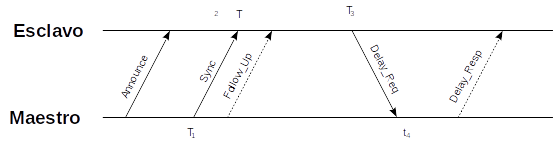
\includegraphics[width=0.7\linewidth]{imagenes/ptp_ts}
	\caption[Intercambio de mensajes para el algoritmo de \acrshort{ptp}]{La 
	figura muestra la secuencia de intercambio de mensajes 
	que se emplea en el algoritmo de \gls{ptp} para conseguir las 4 marcas de 
	tiempo necesarias en el cálculo del \textit{round-trip time} y del desfase.}
	\label{fig:ptpts}
\end{figure}

Para la clase de mensajes generales caben ser destacados los siguientes:

\begin{itemize}
	\item \textbf{Announce} \\
	Es el tipo de mensaje utilizado para informar al resto de los nodos acerca 
	del nodo que transmite (estado y características) además de quién es su 
	\gls{gm}. Son utilizados por el algoritmo \gls{bmc}.
	
	\item \textbf{Follow\_Up} \\
	Sirve para transmitir la marca de tiempo en la escala del maestro para la 
	emisión del mensaje \textit{Sync}.
	
	\item \textbf{Delay\_Resp} \\
	Análogo al anterior para el caso del mensaje \textit{Delay\_Req}.
	
	\item \textbf{Gestión y señalización} \\
	Se engloban mensajes para control y gestión de los relojes o para 
	transmitir información general de estado entre los nodos.
	
\end{itemize}


\subsection{Rendimiento}

Como se ha visto la esencia del mecanismo de sincronización de \gls{ptp} es 
similar al visto anteriormente en la sección de \gls{ntp}: se intercambian una 
serie de paquetes con marcas de tiempo entre dos nodos de la red para calcular 
el desfase entre sus relojes, entonces ¿cómo se consigue la mejora? La gran 
diferencia entre ambos protocolos es la inclusión en el primero del sellado de 
tiempo a nivel de \textit{hardware}. Cuando un paquete de tipo \gls{ptp} llega 
a un puerto, este genera un evento para que una lógica especial realice un 
sellado de tiempo de dicho paquete. Dicha lógica se encuentra entre la capa 
física (PHY) y la capa de enlace (MAC) del modelo \acrshort{osi} 
(\textit{\acrlong{osi}}). Este mecanismo evita la latencia que supone el 
procesamiento de los paquetes y el sellado de tiempo a nivel de 
\textit{software}. Otra diferencia significativa entre \gls{ntp} y \gls{ptp} se 
encuentra en la gestión de las colas de recepción/envío que son fuente de 
retardos no deterministas. Gracias al sellado con soporte \textit{hardware} y 
al tratamiento de los retardos ocasionados por las colas, \gls{ptp} consigue 
una precisión de decenas de nanosegundos con las técnicas más avanzadas 
actualmente. \incomment{referenciar algo}




\section{White Rabbit}

\acrfull{wr} hace referencia tanto al protocolo diseñado como mejora de 
\gls{ptp}v2 como al proyecto internacional que se encarga de su desarrollo y 
mantenimiento. Inicialmente parte como una tecnología desarrollada por el 
\gls{cern} para actualizar el sistema de sincronización y envío de datos de 
control para su complejo de aceleradores de partículas. Gracias a el espíritu 
abierto con el que se desarrolló la tecnología (y a su prometedor rendimiento) 
fueron sumándose otras instituciones al desarrollo, tanto desde el ámbito 
académico, donde cabe destacar el Centro de Investigación de Iones Pesados 
(\textit{Gesellschaft für Schwerionenforschung}, GSI en alemán) en Alemania o 
la propia Universidad de Granada; como desde el empresarial, donde se está 
intentando expandir la tecnología al ámbito industrial. Ejemplos de ello son la 
empresa Seven Solutions (\text{spin-off} de la UGR) en Granada, o CreoTECH en 
Polonia. 

Aunque el empuje en el ámbito de la ciencia es mucho más 
evidente gracias a la inclusión de \textit{WR} en instalaciones para 
aceleradores de partículas, institutos metrológicos o en sistemas de 
adquisición ditribuida como el caso del proyecto Square Kilometre Array (SKA) 
que se está contruyendo en Sudáfrica y que una vez concluido será el 
instrumento de observación astronómica más sensible jamás construido por la 
humanidad. En el caso de la empresa privada, \gls{wr} se ve todavía como una 
tecnología muy prometedora para diversas áreas como Smart Grid, 
Geo-posicionamiento o para las telecomunicaciones, que aún necesita madurar. 
Esto está a punto de cambiar gracias a su inclusión en la próxima revisión del 
estándar \gls{ptp} bajo un nuevo perfil de alta precisión.

Los objetivos de desarrollo iniciales estaban enfocados al entorno de los 
aceleradores de partículas, priorizando una sincronización de calidad junto a 
un sistema que fuese determinista y fácil de mantener:

\begin{itemize}
	\item Lograr para una red de miles de nodos, conectados por enlaces de 
	fibra óptica de hasta 10 km, una diferencia menor del nanosegundo entre dos 
	nodos cualesquiera de la red, es decir, una exactitud de sincronización 
	\textbf{sub-nanosegundo}. Además, se requiere una precisión en el orden del 
	picosegundo.
	
	\item Permitir que el enlace utilizado para los paquetes del protocolo 
	\gls{wr} se pueda \textbf{compartir para} el envío de \textbf{datos de 
	propósito general}, 
	reduciéndo así costes en el despliegue de las infraestructuras.
	
	\item Realizar un desarrollo \textbf{simple y escalable} que no necesite de 
	sofisticados procedimientos de configuración o calibración.
	
	\item Establecer un envío \textbf{determinista} para los paquetes 
	prioritarios, con 
	retardos que no superen ciertos valores umbrales. Esto es especialmente 
	importante en sistemas de control donde la respuesta a un evento no puede 
	exceder un tiempo límite en su envío.
	
	\item Proveer un \textbf{diseño} de referencia \textbf{abierto} a la 
	comunidad 
	(tanto \textit{hardware} como \textit{software}) para fomentar el 
	desarrollo por parte de esta, y evitar las ligaduras con fabricantes.
\end{itemize}

En la actualidad se puede afirmar que en su mayor parte se han cumplido dichos 
objetivos. El requisito principal de rendimiento es algo que se ha conseguido 
en su mayor parte aunque hace falta aportar datos acerca del comportamiento del 
protocolo en redes realmente grandes con un gran número de nodos. La tendencia 
actual en cuanto a rendimiento se centra en la mejora de la exactitud alcanzada 
en escenarios no tan típicos, como enlaces de larga distancia o escenarios con 
cambios en las condiciones de operación. También se investiga como reducir el 
ruido producido por los componentes del sistema de sincronización para lograr 
una precisión en el orden del femtosegundo. El envío determinista es algo que 
no siempre se logra, ya que se puede producir la pérdida de algún paquete de 
alta prioridad en casos de congestión del enlace. Las herramientas de gestión y 
mantenimiento es otro punto al que todavía le queda trabajo por delante y al 
que se está prestando bastante atención dado que son algo crucial si se 
pretende extender el uso del protocolo más allá del ámbito científico.

El protocolo \gls{wr} fue diseñado como una extensión del protocolo IEEE 
1588-2008 (\gls{ptp}v2) al que se añadieron varias mejoras como un modelo de 
enlace más preciso, técnicas de calibración automática o sintonización de los 
relojes mediante el envío de la frecuencia maestra codificada en los paquetes 
transmitidos.



